\chapter{Related work}
\label{chap:rw}

This chapter gives a general overview on how Bitcoin works as well as addressing previous work on both Bitcoin and similar~\acrlong{p2p} systems. Section~\ref{sec:bb} describes the basics of Bitcoin and Blockchain technologies, along with Bitcoin mechanisms for information dissemination. Afterwards, Section~\ref{sec:vulnerabilities} surveys previous work developed on Bitcoin and some of its vulnerabilities.

\section{Bitcoin and Blockchain}
\label{sec:bb}
This section provides an overview of the operation of the Bitcoin network. Bitcoin was created in 2008 by Satoshi Nakamoto with the aim of creating an infrastructure for allowing people to make transactions without depending on a centralized third party while, at the same time, preserving some anonymity~\cite{nakamoto2008bitcoin}. For this purpose, Bitcoin creates a cryptographic currency that can be exchanged among parties. In order to exchange bitcoins, the two parties must own public-/private-keypairs and execute a protocol where the transaction is signed in such a way that serves as a cryptographic proof that the payer paid to the payee~\cite{decker2013information}. A key idea of Bitcoin is that all transactions that involve the exchange of bitcoins between two parties are registered in a serial log that cannot be tampered. This log is built by linking multiple blocks, where each block contains a set of transactions, in an infinite chain known as the \emph{blockchain}. Bitcoin is completely decentralised, and the blockchain is maintained cooperatively by multiple nodes.

In the rest of this section, we provide a more detailed description of several modules of Bitcoin. We start by describing how transactions are represented in Section~\ref{sec:transactions}. Next, we describe how multiple transactions are registered in blocks, that contain the most recent transactions (Section~\ref{sec:blocks}). In Section~\ref{sec:blockchain} we discuss how these blocks are linked together to create the blockchain. Then, in Section~\ref{sec:p2pnetwork} we present how the \acrlong{p2p} network is built and maintained in Bitcoin.
Finally, in Section~\ref{sec:dataexchange}, we describe how information is disseminated throughout the network.

\subsection{Transactions}
\label{sec:transactions}

%Composition of a transaction
A  transaction represents the exchange of currency between accounts. It is composed of inputs, outputs, a transaction ID and other fields not relevant for this work. The inputs are the accounts of the payers, the outputs are the accounts of the payees' and the transaction ID is the hash of the serialised transaction. The transaction ID is also what is used to identify the transaction~\cite{decker2013information}.

%Balance of an account
For an account to be able to spend bitcoins, the nodes responsible for accepting transactions have to know the balance of that account. Nodes know the balance of an account because they keep track of all unspent transactions of that specific account~\cite{decker2013information}. Unspent transactions are transactions where an account received a payment of bitcoins. This means that the account appeared in the array of outputs of those transactions. These transactions are proof that an account has bitcoins; they work like a receipt. 
%Unspent transactions of an account are transactions where the account appears in the array of outputs of those transactions, meaning that the owner of that account was paid the amount of Bitcoins that he now owns.

%How can a transaction be confirmed
In order for a transaction to be valid, the payers have to sign the transaction. This means that each owner transfers the amount to the payee by digitally signing a hash of the previous transaction and the public key of the payee as seen in Figure.~\ref{fig:signature}~\cite{nakamoto2008bitcoin}. The previous transaction is the transaction where the current payer received the bitcoins that he is using in the current transaction.

\begin{figure}[h]
\centering
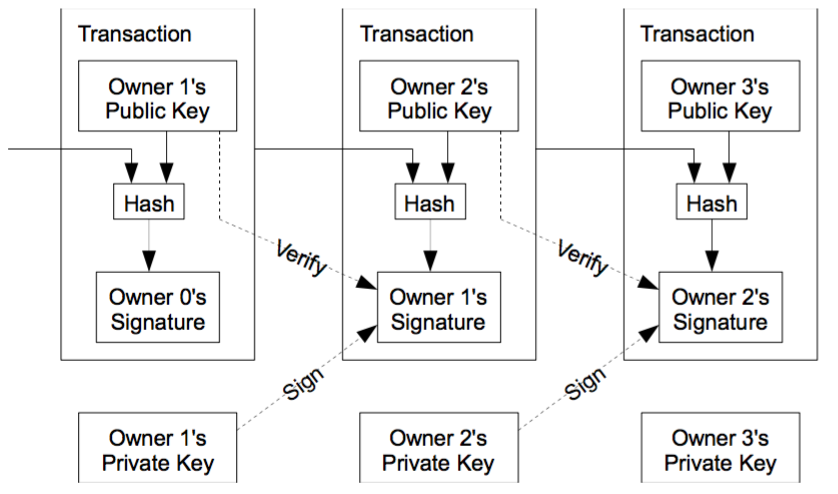
\includegraphics[scale=0.5]{figs/transactions}
\caption{Signing mechanism. Original from~\protect\cite{nakamoto2008bitcoin}}
\label{fig:signature}
\end{figure}

Furthermore, transactions have to fulfil the following criteria regarding outputs they claim and create in order to be valid~\cite{decker2013information}:
\begin{itemize}
  \item An output may be claimed at most once;
  \item Outputs are created solely as a result of a transaction;
  \item The sum of the values of the claimed outputs has to be greater or equal than the sum of the values of the newly allocated outputs. Claimed outputs are bitcoins the payer is trying to spend and allocated outputs are the amount of bitcoins the payee accounts are going to be able to spend. For instance, if user \textsl{A} and \textsl{B} want to buy a product to \textsl{C} that costs $3$ bitcoins where each one contributes with $1.5$ bitcoins in the claimed outputs will appear two entries each of $1.5$ bitcoins and in the newly allocated resources have to be exactly $3$ bitcoins, or less, as some amount can be claimed by the miners as a tax for including the transaction in the block.
\end{itemize}

The first criteria exist so that the user cannot double spend bitcoins. The second ensures that unspent bitcoins need to be connected to a transaction, avoiding forging of unspent bitcoins. The third guarantees that bitcoins can only be transferred and not created.

In order for payees to know that previous owners did not sign any earlier transactions, transactions are broadcasted through the Bitcoin network~\cite{nakamoto2008bitcoin}. This feature is required to ensure the payee that the payer did not already spend the bitcoins he is using to pay him. However, this feature introduces inconsistencies in the system, as transactions reach different nodes at different times:
\begin{itemize}
    \item A node could receive a transaction that transfers bitcoins from owner \textsl{B} to owner \textsl{C}, however that node has yet to receive the transaction that transferred the bitcoins from owner \textsl{A} to owner \textsl{B}. As a result the transaction might not being accepted or it might take a longer time to be accepted;
    \item A node could also receive two transactions from the same owner \textsl{A} where he tries to transfer the same bitcoins to two different payees \textsl{B} and \textsl{C}. This is a case of double-spending.
\end{itemize}

As there is no guarantee that different nodes receive conflicting transactions in the same order, those nodes will disagree on those transactions and any transactions built on top of them by claiming their outputs~\cite{decker2013information}. This would have been a problem because they would not agree upon a common record. For instance, if a user \textsl{Joe} sent his transaction to node \textit{A}, \textit{A} would accept it because in its record \textsl{Joe} had those bitcoins to spend. But if \textsl{Joe} had sent his transaction to node \textit{B}, \textit{B} might not have accepted it because in its record \textsl{Joe} had never been the owner of the bitcoins he is trying to transfer. We will see how this problem is solved by Bitcoin in the next section.

\subsection{Blocks}
\label{sec:blocks}

Since different nodes can process and even commit transactions in a different order they need to have a way to reach a consensus on the set of transactions that are considered valid. The role of the blocks is precisely to allow nodes to agree upon a set of transactions.

Each block is composed of a set of transactions, a nonce, a pointer to its parent block and other fields not relevant for this explanation. Each block is also associated with a block header that summarises the information in that block.

In order for a block to be accepted by other nodes it has to present a~\acrlong{pow} (\acrshort{pow}). \acrshort{pow} consists in finding a byte string, called nonce, that hashed with the block header results in a hash with a given number of zeros at the beginning. That number of zeros at the beginning is also called \textit{target}~\cite{decker2013information}. As cryptographic hash functions are only one-way, discovering such nonce can only be done by trial and error. Furthermore, the difficulty of the \textit{target} is also adjusted as follows. The Bitcoin network measures how much time it took to create the last $2016$ blocks in a blockchain. If it took significantly more than $2$ weeks, the \acrshort{pow} difficulty is reduced, meaning that there will be fewer zeros at the beginning of the next \textit{target}. If it took significantly less than $2$ weeks, the difficulty is increased. 

The \acrshort{pow} is necessary because it adds a real-world cost to produce a block. So with the requirement of a block having to present a \acrshort{pow}, it becomes infeasible for people to modify the history of the system and present it as the truth to anybody else as we will see in Section~\ref{sec:51attack}.

To incentivise miners for having spent resources on finding the \acrshort{pow}, each time a new block is created a new Bitcoin is generated~\cite{decker2013information}. The reward transaction is only valid if it appears in a block. This transaction is also the only transaction that is the exception to the third criteria seen in the Section~\ref{sec:transactions} which states that the sum of the inputs has to be greater or equal to the sum of the outputs~\cite{decker2013information}.

Today as the number of transactions increases on a daily basis and given the limited space each block has for transactions (1MB), miners also profit through fees imposed on transactions. Most miners choose which transactions to include in their blocks based on how profitable they expect those transactions to be. If there are two transactions of equal byte size but only one of them fits in a block, then the miner will choose whichever transaction has the higher transaction fee.

Due to the very low probability of successful generation, it is unpredictable which miner nodes in the network will be able to generate the next block. Hence, when a node finds a new block, it broadcasts it to the other nodes. Upon receiving a new block, two things can happen:
\begin{itemize}
\item The node will rollback all tentatively committed transactions since the last block reception and then commit the ones on the new block~\cite{decker2013information}. Tentatively committed transactions are transactions that were valid and would have been committed if the node had been able to generate a new block.
\item The node has already mined or received a new block and it will ignore the newly received block. The implications of this are further discussed in Section~\ref{sec:blockchain}.
\end{itemize}
%At this point, all nodes have agreed on the validity of all transactions on the block \cite{decker2013information} and the network has been synced.

Regarding the tentatively committed transactions that were rolled back, if they were present in the new block they do not have to be re-applied. For the tentatively committed transactions that were not, they will be re-applied only if they are valid as conflicting transactions might have been present in the newly received block. Invalid transactions are transactions that conflict with one or more transactions that were present in the new block. If a transaction is flagged as invalid it will be discarded~\cite{decker2013information}. The node that created the invalid transaction will eventually receive the block with the valid transaction and it will have to rollback the invalid transaction.

Because of this feature, the creator of the block imposes which transactions are going to be committed and what is the order that they are committed~\cite{decker2013information}.

In the next section, we will see how blocks are linked together to create a distributed record of what happened.

\subsection{Blockchain}
\label{sec:blockchain}
As we have seen, blocks are used by nodes to agree on the order of recent transactions. Furthermore once a block is generated it is also linked with the block that preceded it. This creates a chronological order over all blocks and therefore transactions as seen in Figure.~\ref{fig:blocks}. This chain of blocks is called \textit{blockchain}~\cite{decker2013information}. The first block in the chain is called the genesis block.

\begin{figure}[h]
\centering
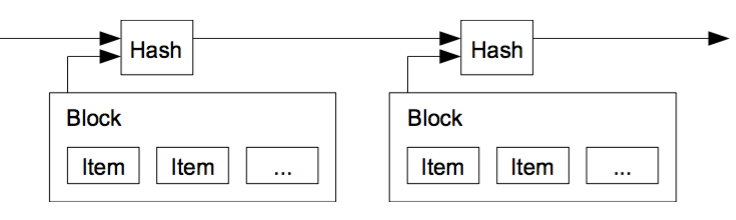
\includegraphics[scale=0.65]{figs/orderBlocks}
\caption{Blockchain representation. Original from~\protect\cite{nakamoto2008bitcoin}}
\label{fig:blocks}
\end{figure}

The blockchain is defined as the longest path from any block to the genesis block. This definition makes the blockchain resemble a tree where the root is the genesis block and the leaves are the new blocks. The height of a block is the distance of that block to the genesis block. The block that is the furthest away from the genesis block is called the blockchain head~\cite{decker2013information}.

As only new blocks are rewarded with new bitcoins, miners try to build on top of the blockchain head~\cite{decker2013information}. This is because if they were to build on top of previously found blocks it would require them to first reach the same height as the blockchain head and then find the new block~\cite{nakamoto2008bitcoin}. This is very hard to do because they would have to remine all the previous \acrshort{pow} and a new \acrshort{pow} while competing against the rest of the computational power present in the network. However, given the resources necessary to find only one \acrshort{pow}, the miners would have to have more computational power than the rest of the network when they first started the fork. Namely, for a miner to have success at doing this he would have to control at least 51\% of the computational power in the network, we will further discuss this in section~\ref{sec:51attack}.

As seen in Section~\ref{sec:blocks}, a node can accept a new block or ignore it. Because of this, there might be multiple blocks at the same height at any point in time. This is called a \textit{blockchain fork}. Hence, when this happens the network does not agree on which block is the blockchain head. This leads to inconsistency of the system because both block \textit{b} and block \textit{b'} are guaranteed to disagree on some transaction, for instance they will always disagree on the reward transaction. This will go on until one of the branches overtakes the other~\cite{decker2013information}.

When a node has as blockchain head block \textit{b} and it receives a new block \textit{b'} where the height of \textit{b' \textgreater b} two things can happen depending on which branch \textit{b} is in:
\begin{itemize}
\item If \textit{b} is in the same branch as \textit{b'}, meaning that \textit{b} is one of the predecessors of \textit{b'}, then the node only has to apply all transactions in the intermediate blocks incrementally, if any, and then apply the transactions in \textit{b'}. Intermediate blocks are blocks that might have been generated after \textit{b} but before \textit{b'}.
\item If \textit{b} is on another branch, meaning that \textit{b} is not a predecessor of \textit{b'}, then the node is required to change branches. This implies that the node has to revert all transactions it has been committing until it reaches a common block ancestor. Then, it has to request all intermediate blocks apply the transactions in those blocks and finally apply the transactions on \textit{b'}~\cite{decker2013information}.
\end{itemize}

The fork may be prolonged throughout multiple block heights \textit{h, h+1, h+2...} where subsets of the network work on the different branches and try to find new blocks at the same time. Eventually one of the branches will surpass the others, leading to the adoption of this branch by all the nodes and therefore the end of the fork~\cite{decker2013information}. The discarded blocks are called \textit{orphan blocks}.

As a consequence of blockchain forks, a transaction in Bitcoin is never committed permanently. Because at any point in time it could appear a branch that was not known by the nodes we were interacting with which might influence the state of our transactions. If this new branch is taller than the one where our transactions were confirmed then our transactions will be rolled back.


%\subsection{Network}
%\label{sec:network}
%Bitcoin is supported by a network of peer-to-peer nodes that mine new Bitcoins, create and disseminate transactions and keep a record of what transactions happened. This network has two components that should be looked into to understand some of the vulnerabilities that we will study in the next section. Those two components are:

%\begin{enumerate}
%	\item Network overlay - how the Bitcoin peer-to-peer network is built;
%	\item Information propagation - how does the Bitcoin protocol forward information.
%\end{enumerate}

\subsection{Overlay Network}
\label{sec:p2pnetwork}

Peers in the Bitcoin network are identified by their IP addresses. A node with a public IP can initiate up to eight outgoing connections with other Bitcoin nodes and accept up to 117 incoming connections. A node with a private IP only initiates eight outgoing connections. Connections are over TCP. Nodes only propagate and store public IPs~\cite{heilman2015eclipse}.

When a node wants to join the network there are five ways for it to connect with peers~\cite{bitcoinwiki}:

\begin{enumerate}
	\item Address database - this local file contains other nodes that the node already knew about. The node will try to re-connect with those nodes. If it is the first time the node connects to the network this method doesn't work;
	\item User-specified - in this method the user can specify nodes to connect to on the command line;
	\item DNS seeding - this option is only used if the Address database file is empty and the user did not specify any nodes. The nodes issue DNS requests to a list of 6 DNS servers that are hardcoded in order to discover IP addresses of other peers, each DNS server can return up to 256 IP addresses;
	\item Hard-coded nodes - If DNS seeding fails, the node contains a list of 1525 hard-coded IP addresses that represent Bitcoin nodes that it contacts to get addresses of other peers and then finishes the connection with them to avoid overloading those nodes;
	\item From other nodes - Nodes exchange IP addresses with other nodes via the \textit{GetAddr} and \textit{Addr} messages which we will discuss later.
\end{enumerate}

\subsubsection{Storing Network Information}
Public IPs are stored in a node’s \emph{tried} and \emph{new} tables.

\paragraph*{\emph{Tried} Table}
The \emph{tried} table consists of 256 buckets, each of which can store up to 64 unique addresses for peers to whom the node has successfully established an incoming or outgoing connection. Along with each stored peer’s address, the node keeps the timestamp for the most recent successful connection to this peer.
Each peer’s address is mapped to a bucket in the table by taking the hash of the peer’s (a) IP address and (b) group, where the group defined is the /16 IPv4 prefix containing the peer’s IP address. We insert the IP in a bucket by first getting a bucket using Algorithm~\ref{alg:triedbucket} and then getting a position inside the bucket using Algorithm~\ref{alg:posinbucket}.

\begin{algorithm}
\begin{algorithmic}[1]
\Function{get\_tried\_bucket}{}
\State SK = random value chosen when node is bootstrapped.
\State IP = the peer’s IP address and port number.
\State Group = the peer’s group
\State
\State i = Hash( SK, IP ) \% 8
\State Bucket = Hash( SK, Group, i ) \% 256
\State \Return Bucket
\end{algorithmic}
\caption{Get bucket in \emph{tried} table for a specific IP}
\label{alg:triedbucket}
\end{algorithm}


\begin{algorithm}
\begin{algorithmic}[1]
\Function{position\_in\_bucket}{Bucket}
\State SK = random value chosen when node is bootstrapped.
\State IP = the peer’s IP address and port number.
\State New = Either ‘N‘ or ‘K’ if we are looking for a position in New or Tried bucket.
\State
\State PosInBucket = Hash(SK, New, Bucket, IP) \% 64
\State \Return PosInBucket
\end{algorithmic}
\caption{Get position of IP inside a specific bucket}
\label{alg:posinbucket}
\end{algorithm}

Thus, every IP address maps to a position in a single bucket in \emph{tried}, and each group maps to up to eight buckets. When a node successfully connects to a peer, the peer’s address is inserted into the appropriate position in the \emph{tried} bucket. If the position already has an address then the node will briefly attempt to connect to the older address, and if connection is successful, then the older address is not evicted from the \emph{tried} table; the new address is stored in \emph{tried} only if the connection fails. If the peer’s address is already present in the bucket, the timestamp associated with the peer’s address is updated. The timestamp is also updated with the local time when an actively connected peer sends a \textsl{Version, Addr, Inv, GetData or Ping} message and more than 20 minutes elapsed since the last update.

\paragraph*{\emph{New} Table}
The \emph{new} table consists of 1024 buckets, each of which can hold up 64 addresses for peers to whom the node has not yet initiated a successful connection. A node populates the \emph{new} table with information learned from the DNS seeders, or from \textsl{Addr} messages. Addresses in the \emph{new} table also have an associated timestamp; addresses learned from DNS seeders are stamped with a random timestamp between 3 and 7 days old. Whereas addresses learned from \textsl{Addr} messages are stamped with their timestamp from the \textsl{Addr} message plus two hours.
Every address \textsl{a} inserted in \emph{new} belongs to (1) a \textsl{group}, defined in the description of the \emph{tried} table, and (2) a \textsl{source group}, the group that contains the IP address of the connected peer or DNS seeder from which the node learned address \textsl{a}. We insert an IP in a bucket by first getting a bucket using Algorithm~\ref{alg:newbucket} and then getting a position inside the bucket using Algorithm~\ref{alg:posinbucket}.

\begin{algorithm}
\begin{algorithmic}[1]
\Function{get\_new\_bucket}{}
\State SK = random value chosen when node is bootstrapped.
\State Group = /16 containing IP to be inserted.
\State Src\_Group = /16 containing IP of peer sending IP.
\State
\State i = Hash( SK, Src\_Group, Group ) \% 64
\State Bucket = Hash( SK, Src\_Group, i) \% 1024
\State \Return Bucket
\end{algorithmic}
\caption{Get bucket in \emph{new} table for a specific IP}
\label{alg:newbucket}
\end{algorithm}

Each (group, source group) pair hashes to a single \emph{new} bucket, while each group selects up to 64 buckets in \emph{new}. Each bucket holds up to 64 addresses like the \emph{tried} table. If a position in a bucket is already occupied by other address then a function \textsl{isTerrible} is invoked. If the other address is terrible, in that it is (a) more than 30 days old, or (b) has had too many failed connection attempts, then the terrible address is evicted in favour of the new address; otherwise, the new address is discarded. A single address can map to multiple buckets if it is advertised by multiple peers; so if the other address is already in multiple buckets we prioritise the new address if the new address is not already in a bucket.

\subsubsection{Propagating Network Information}

Network information propagates through the Bitcoin network via DNS seeders and \textsl{Addr} messages.
\paragraph*{DNS seeders}
A DNS seeder is a server that responds to DNS queries from Bitcoin nodes with a (not cryptographically-authenticated) list of IP addresses for Bitcoin nodes. The maximum possible number of IP addresses that can be returned by a single DNS query is 256. The seeder obtains these addresses by periodically crawling the Bitcoin network. The Bitcoin network has six seeders which are queried in two cases only~\cite{heilman2015eclipse}.
\begin{itemize}
  \item When a new node joins the network for the first time; it tries to connect to the seeders to get a list of active IPs, and otherwise fails over to a hardcoded list of 1525 IP addresses.
  \item When an existing node restarts and reconnects to new peers, the seeder is queried only if 11 seconds have elapsed since the node began attempting to establish connections and the node has less than two outgoing connections.
\end{itemize}

\paragraph*{Addr Messages}
\textsl{Addr} messages, containing up to 1000 IP addresses and their timestamps, are used to obtain network information from peers. If more than 1000 addresses are sent in a \textsl{Addr} message, the peer who sent the message is blacklisted. Nodes accept unsolicited \textsl{Addr} messages. An \textsl{Addr} message is only solicited by a node upon establishing an outgoing connection with a peer, the peer responds with the \textsl{Addr} containing up to 1000 addresses randomly selected from its tables. The peer sends a total of \textsl{n} randomly selected addresses from the peer’s \emph{tried} and \emph{new} tables, where \textsl{n} is a random number between \textsl{x} and 2500, where \textsl{x} is 23\% of the addresses the peer has stored~\cite{heilman2015eclipse}.

Nodes push \textsl{Addr} messages to peers in two cases. Once a day, a node sends its own IP address in a \textsl{Addr} message to each peer. Also, when a node receives an \textsl{Addr} message with no more than 10 addresses, it forwards the \textsl{Addr} message to two randomly-selected connected peers. Actually, if the \textsl{Addr} message contains addresses that are unroutable for the peer (e.g., a peer with IPv4 address gets an IPv6 address), it will forward the \textsl{Addr} message to one peer only. To choose these peers, the node takes the hash of each connected peer’s IP address and a secret nonce associated with the day, selects the peers with the lexicographically first and second hash values.

Finally, to prevent stale \textsl{Addr} messages from being endlessly propagated, each node keeps a known list of the addresses it has sent to or learned from each of its connected peers, and never sends address on the known list to its peer. The known lists are flushed daily.


\subsubsection{Selecting Peers}
New outgoing connections are selected if a node restarts or if an outgoing connection is dropped. A Bitcoin node never deliberately drops a connection, except when a blacklisting condition is met (e.g., the peer sends \textsl{Addr} messages that are too large).
A node with $\omega \in [0,7]$ outgoing connections selects the $\omega+1th$ connection as follows:
\begin{enumerate}
  \item Decide whether to select from \emph{tried} or \emph{new} tables with a $50\%$ probability.
  \item Select a random address from the table, with a bias towards addresses with fresher timestamps: 
  \begin{itemize}
      \item (i) Choose a random non-empty bucket in the table.
      \item (ii) Choose a random position in that bucket.
      \item (iii) If there is an address at that position, return the address with probability:
  \end{itemize}  
  \begin{equation}
    p(r, \tau) = min(1, \dfrac{1.2^{r}}{1+\tau})
  \end{equation}
  else, reject the address and return to step (i). The acceptance probability $p(r, \tau)$ is a function of $r$, the number of addresses that have been rejected so far, and $\tau$, the difference between the address’s timestamp and the current time in measured in ten minute increments.
  \item Connect to the address. If connection fails, go to (1).
\end{enumerate}

\subsubsection{Feeler Connections}
An outgoing connection that establish short-lived test connections to randomly selected addresses in \emph{new}. If connection succeeds, the address is evicted from \emph{new} and inserted into \emph{tried}; otherwise, the address is evicted from \emph{new}. Feeler connections clean trash out of \emph{new} while increasing the number of fresh address in \emph{tried} that are likely to be online when a node restarts.

\subsubsection{Mining Pools}
There are also organisations called \textit{mining pools}, composed by multiple nodes that work together to find the \acrshort{pow} more efficiently. In mining pools, each node tests different nonces to find the \acrshort{pow} which is faster than a single node testing all the possible nonce's. \textit{Mining pools} are composed by multiple nodes and gateways that connect the pool to the Bitcoin network. Once they find a \acrshort{pow} and generate a block the reward is then split among the members of the pool that worked on that \acrshort{pow} proportionately to the contribution that each member made. Accordinging to \url{blockchain.info} currently around $89.2\%$ of the blocks created come from mining pools.

\subsection{Information propagation}
\label{sec:dataexchange}
In order to exchange messages, Bitcoin nodes maintain for each of its neighbours, a message queue that is used to push the different types of messages. Then all the messages in the queue will be sent once a timer associated with the queue timeout. The timeout is calculated using a Poisson distribution that has in consideration if the neighbour is outbound or inbound and attributes higher timeouts to inbound nodes.

\subsubsection{Transactions}
Transactions are usually relayed to other nodes through advertisements as follows.

Node \textit{A} creates a new transaction, and add the advertisement for that transaction to the message queue of all its neighbours. If \textit{A} learns, from advertisements that its neighbours send, that one of its neighbours already has that transaction, it will remove the advertisement for that transaction from the queue of that neighbour. When the timer associated with the queue of, for instance, the neighbour \textsl{B} times-out, \textsl{A} will send all the advertisements in the queue to \textit{B} in the format of an \textsl{Inv} message. Once \textsl{B} receives the \textsl{Inv} message, it will check if it already has all the transactions in the advertisement, after going through all advertisements, \textit{B} will then send to \textsl{A} a \textsl{GetData} message requesting all the transactions advertised that it currently does not has in his \emph{mempool}, structure where nodes save all the transactions that have not yet been added to a block. After receiving the \textsl{GetData} message, \textit{A} will then add the requested transaction individually in a \textsl{TX} message to the queues of the neighbours that requested it. Finally, once \textsl{B} receives the new transaction it will verify if it is valid and if it is, it will also relay it through his neighbours.

However, transactions can also be relayed to other nodes in two other ways, direct push or \textsl{BlockTX} messages. In direct push the transaction is sent directly to the other nodes. However \textsl{BlockTX} messages are only sent to reply to \textsl{GetBlockTX} messages that nodes send when they received a compact block and do not have all the transactions necessary to rebuild the block as explained in the next paragraph.

\subsubsection{Blocks}
Until Bitcoin version 0.13.0 (23-08-2016) the usual way to relay blocks was also through advertisements, similar to the way transactions are relayed. However, with the addition of a new message type, compact block \textsl{CMPCTBlock}, the mechanism for relaying blocks changed a bit.

The difference between a block message and a compact block message is that the block message contains not only the header of the block but also all the transactions present in that block, whereas, the compact block message only contains the header of the block and the ids and the index of the transactions present in that block. Another difference is that once a node receives a compact block it has to rebuild the block and validate it before relaying it. Hence the main advantage of the compact block over the block message is the lower amount of bandwidth consumed to send a block. Because of this, nowadays the main method for relaying a block between up to date nodes is through compact blocks. However if, a node receives a block with ids that it does not know, it has to send to the neighbour that sent him the block a \textit{GetBlockTX} message requesting the transactions it is missing. Finally, once a node receives a \textit{GetBlockTX} it will respond with a  \textit{BlockTX} message containing all the missing transactions~\cite{bip152}.

This means there are in total tree ways a block can be relayed as we can see in Figure.~\ref{fig:protocol-flow}. In this figure we can see how the protocol behaves in the legacy relaying in A we can also see the two new ways to disseminate information. The ones described previously was A and B. In~\cite{bip152} the author claims that a Bitcoin node would use the protocol described in C to disseminate blocks if it had low bandwidth but during the tests we did and the inspections we did to the source code we never saw this protocol being used.

\begin{figure}[h]
\centering
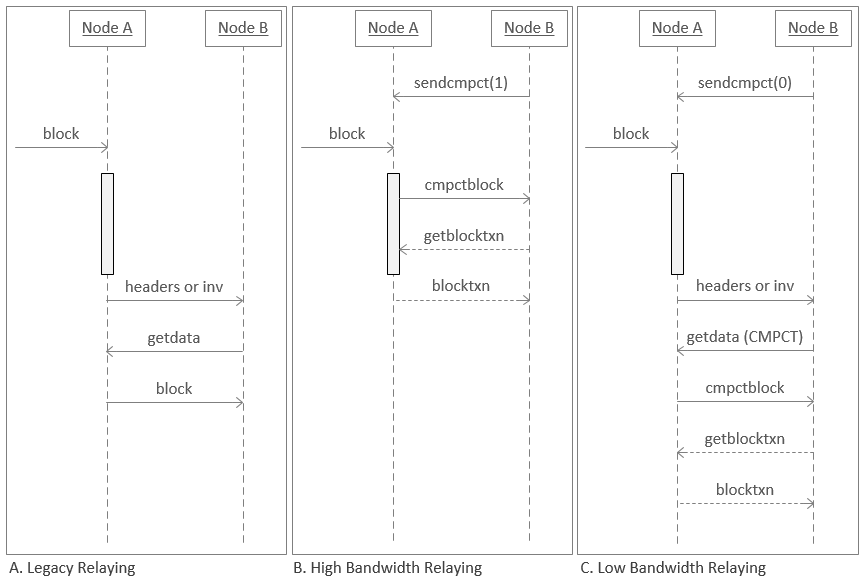
\includegraphics[scale=0.5]{figs/bip-152.png}
\caption{Protocol Flow (Source Matt Corallo)}
\label{fig:protocol-flow}
\end{figure}

There are also messages that allow, nodes that were disconnected from the network, to quickly get the data that they have missed. These messages are especially useful to speed up the process of gathering data for the creation of blocks. They are also useful when nodes do not have the parent block of a block they just received. In this case, they can use these messages to ask their neighbours for the missing block \cite{bitcoincorewiki}.

\subsection{Summary}
In conclusion, Bitcoin is a very complex system with many modules and libraries that allow it to work properly. However, in this thesis, we were mainly focused on improving its dissemination system. From the point of view of our work, the most important modules are depicted in Figure~\ref{fig:bitcoinoverview}. We will now briefly describe each component.

\begin{figure}[h]
\centering
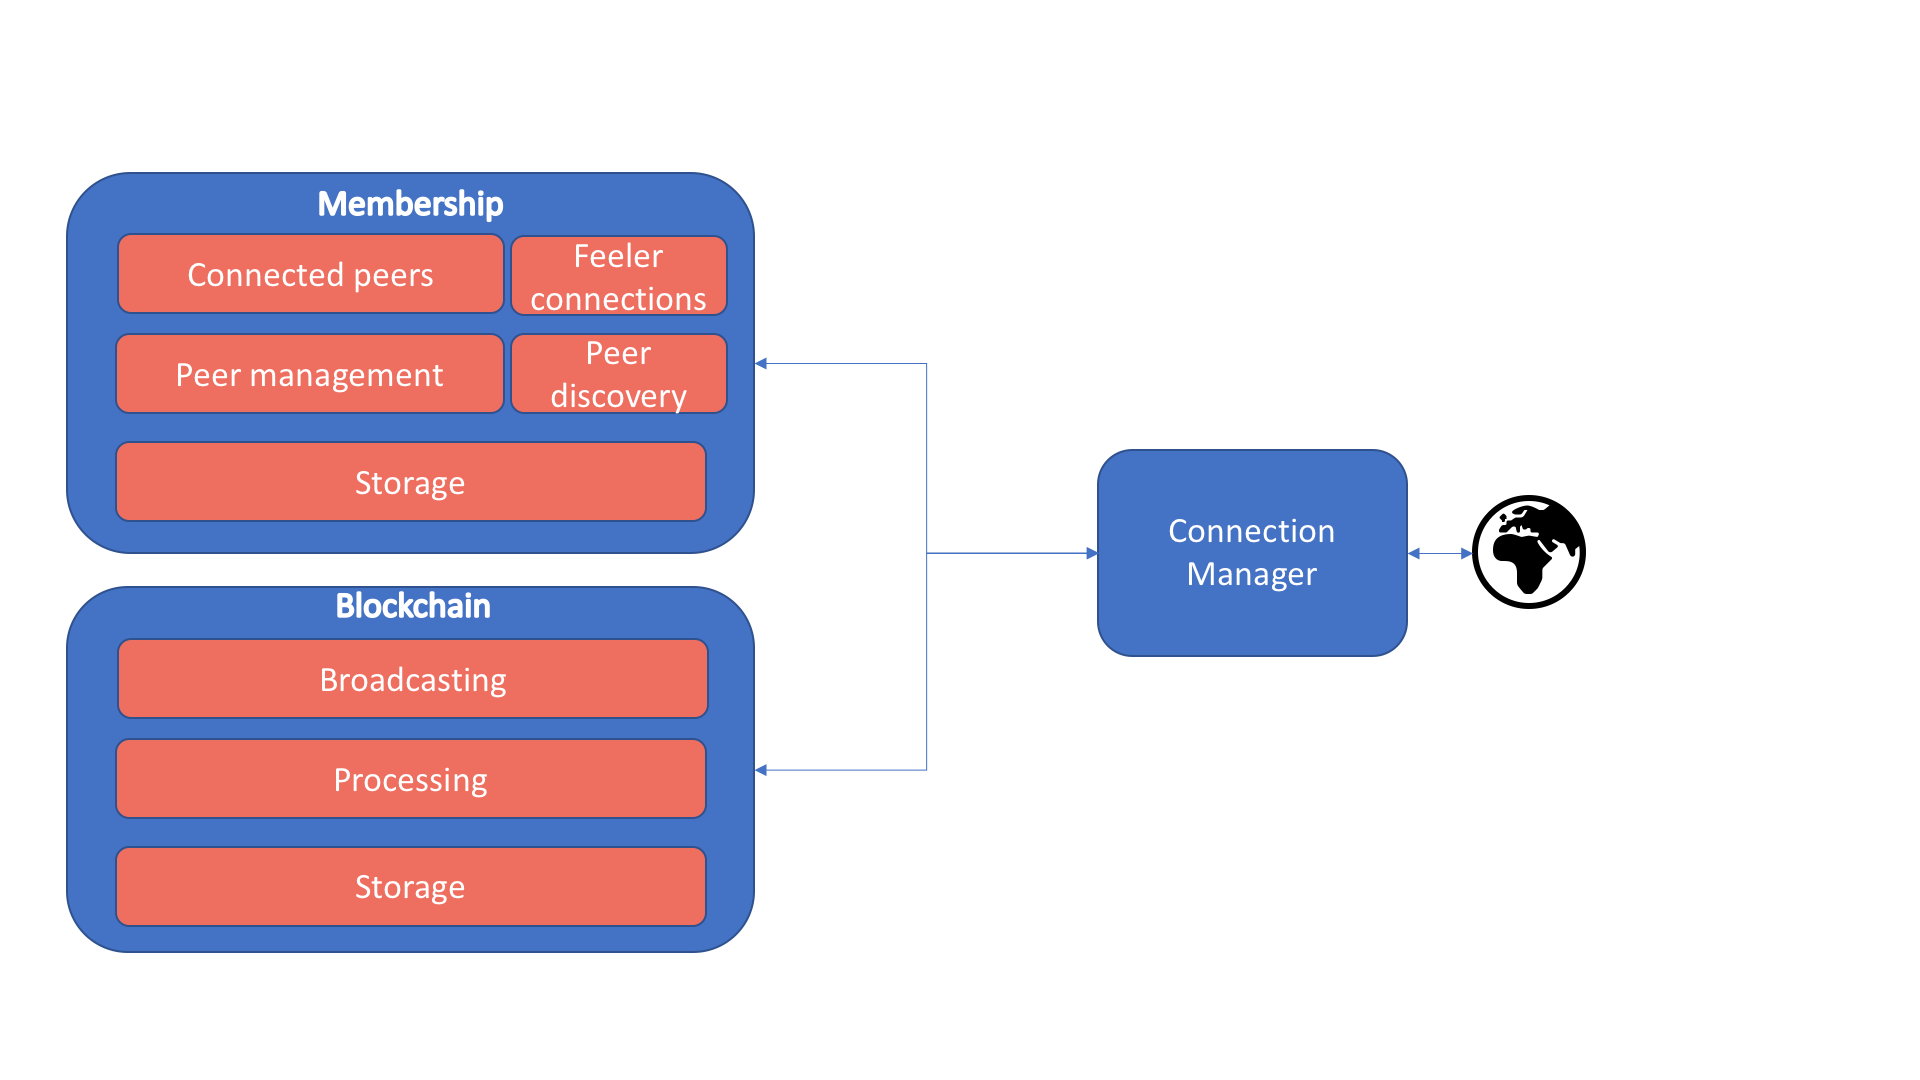
\includegraphics[scale=0.4]{figs/My-Bitcoin-Core-architecture}
\caption{Bitcoin architecture}
\label{fig:bitcoinoverview}
\end{figure}

Starting with the Blockchain module, this module is responsible for every operation related to the blockchain, from receiving transactions and validating them to broadcasting blocks. This module is composed mainly of three sub-modules, the broadcasting module, the processing module and storage module. We will now go over each individual module:
\begin{itemize}
    \item \textbf{Broadcasting module} is responsible for broadcasting/receiving blockchain information to/from the current neighbours of a node;
    \item \textbf{Processing module} is in charge of validating every transaction and block a node receives;
    \item \textbf{Storage module} stores all information necessary to maintain the blockchain.
\end{itemize}

Regarding the membership, this module it is composed of four modules the connected peers and the feeler connections, a peer management module and a storage module.
\begin{itemize}
    \item \textbf{Connected peers module} as the name suggests is the set of peers currently connected to a node;
    \item \textbf{Feeler connections module} are the connections described at the end of Section~\ref{sec:p2pnetwork};
    \item \textbf{Peer management module} is responsible for managing each peer and check if they should be banned or not.
    \item \textbf{Peer discovery module} is in charge of finding new peers to connect to;
    \item \textbf{Storage module} is responsible for storing information about each connected peer and as well as the \emph{tried} and \emph{new} tables.
\end{itemize} 

Finally, the connection manager is in charge of establishing the low level connections between the peers.

Next, we will take a look at some of the vulnerabilities of some of the modules of Bitcoin to understand which modules have to be modified in order to fix those problems.


\section{Bitcoin and Blockchain Vulnerabilities}
\label{sec:vulnerabilities}
In this section, our objective is to analyse known vulnerabilities in some of the aforementioned modules. Hence, this section is divided into two sub-sections, in Section~\ref{sec:b_module} we will present vulnerabilities related with the blockchain module and Section~\ref{sec:m_module} we will discuss vulnerabilities related with the membership module.

\subsection{Blockchain Module}
\label{sec:b_module}

In this subsection, we will cover known vulnerabilities of the blockchain module in Bitcoin.

\subsubsection{Information Broadcast Module}
\label{sec:info_broad_module}

We will now describe three vulnerabilities in this module: information eclipsing, block delay and double-spending.

Starting with information eclipsing, this vulnerability happens because of the following behaviour. Lets consider that the whole network recognises a block \textsl{b} at height $H_b$ as the blockchain head. Then at two different locations of the network two new blocks are discovered. These blocks are guaranteed to be different as seen in Section~\ref{sec:blocks}, lets call each one \textit{b'} and \textit{b''}~\cite{decker2013information}.

Now both blocks are going to be broadcast through the network because both are at height $H_{b+1}$. Hence, when a node receives either \textit{b'} or \textit{b''} it will consider it as the new blockchain head and will broadcast it to its neighbours. The problem is, when a node that already received \textit{b'} receives \textit{b''} or vice-versa that node will not broadcast \textit{b''} through the network as it did with \textit{b'}, because it already moved to a new blockchain head at the same height. As a consequence, only nodes that received both \textit{b'} and \textit{b''} know about the existence of a fork. This diminishes the effective computational power in the network because the network will be working on different blockchain heads. Hence, empowering some of the attacks in the following sections.

The authors of the paper discovered that it takes 6.5 seconds for the block reach 50\% of nodes, 40 seconds for it to reach 95\% of nodes and that the mean delay for a block to reach a node in the network is 12.6 seconds. Since Bitcoin has a block creation time of 10 minutes the authors concluded that the effective computational power in the Bitcoin network is only 98.20\%. This happens because once a block is found it takes in mean 12.6 seconds for it to reach a node, so during those 12.6 seconds the rest of the network is wasting resources (resources that do not contribute to extend and strengthen the blockchain).

If we wanted to use Bitcoin for faster transactions, then the block dissemination time would have to go down. But if we maintain the 12.6 propagation delay and decrease the block dissemination time the effective computational power would also decrease even more as showcased in~\cite{ethereumblog}. The intuition is that with a lower block time the probability of stale blocks\footnote{Blocks that were candidates to being the next blockchain head but were not chosen.} being created increases. This will result in more forks being created and more resources more wasted resources.

%Regarding solutions, the authors suggested multiple options to optimize the propagation of a block, which would lower the 12.6 seconds delay and the lower probability of stale blocks being created. One of the solutions consisted in changing the block verification process. In this solution, the verification of a block would be split into two phases an initial difficulty check and a transaction validation. Since the transaction validation is the phase which takes longer, a node would perform the initial difficulty check where it checks the validity of the \acrshort{pow} and once this was done the node could broadcast the \textit{Inv} messages right away while performing the transaction validations asynchronously.

It is worth noting that the problem identified in this work is worth revisiting as the protocol for block dissemination has evolved considerably over the years, for instance, with the introduction of compact blocks which implements some of the ideas proposed in~\cite{decker2013information}. Furthermore, at the time of this writing, according to \url{blockchain.info} there have only been five instances of soft forks in 2018, meaning that two blocks were created at the same height.

%Ethereum solved part of this problem through the implementation of uncle blocks. Rather than discarding stale blocks as in Bitcoin, Ethereum includes them in new blocks, hence the name uncle blocks. Uncle blocks are included in new blocks up to a certain height difference between the uncle block and the new block being generated. This happens because nodes that generated uncle blocks are rewarded with a fraction of the full reward, so the limit imposed by the height difference avoids having a group of nodes mining on lower heights.

%With this solution Ethereum solved this problem because now blocks to be built also include other previously built blocks in addition to the already included parent block. This means that no computational power is lost. Because for an attacker to forge a block he would need to remake all previous blocks of the main chain and all the uncle blocks of that block, since uncle blocks also had the transaction that the attacker is trying to eliminate. This attack is further explained in the next section.

%The disadvantage of this solution is the extra computational power and memory required to include the uncle blocks.


The block delay vulnerability is based on slowing down the propagation of new blocks sent to a set of nodes without disrupting their connections~\cite{apostolaki2016hijacking}. This attack takes advantage of a specific condition where nodes wait 20 minutes before requesting a block to another node if the node how advertised the block did not reply with the block requested.

This vulnerability, called block delay, has two different ways of being performed depending on the direction the attacker is able to intercept the traffic: in the victim network \textit{V$\,\to\,$N} direction or network victim \textit{N$\,\to\,$V} direction.

If the attacker is able to intercept the connection in the \textit{V$\,\to\,$N} direction then the attack works as follows. When the victim requests a block to the network the attacker will change the block request to another block which will lead the victim waiting for a response. After almost 20 minutes, time limit where the victim requests the block to another neighbour, the attacker will modify another message sent by the victim to that neighbour, probably a transaction request since are the most common message type, to request the initial block that the victim wanted. This way the attacker avoids the victim from dropping the connection with that neighbour, which allows the attacker to perform the attack multiple times.

If the attacker is able to intercept the communication in the other direction \textit{N$\,\to\,$V}. In this direction, once the victim requests a block to a neighbour the attacker will intercept and tamper with the response (the block itself) corrupting it, which will lead to it being discarded by the victim. But the victim will not request the corrupted block again. Then, after 20 minutes the victim will drop that connection because the block never arrived and will request the block to another neighbour. Hence, the attack performed this way can only be done once.

The impact of this attack depends on the node that is being attacked. If it's a common node, like the one a normal person would run, then this attack will be a Denial of Service and that node will not have guarantees for double spending. However if that attack is towards a gateway of a pool it could be used to engineer block races, block races will be further discussed in Section~\ref{sec:selfish}.

A solution for this attack is monitoring the RTT of the block requests, as the RTT increases considerably when the node is being attacked. Other solution proposed in~\cite{apostolaki2016hijacking} is encrypting Bitcoin communications which would not avoid the packets from being dropped by an attacker but it would prevent them from eavesdropping and tampering with connections. The disadvantage with this approach is that it would require additional computations making the system slower.

%Ethereum and Ripple are not affected by this attack as all the connections are encrypted but the attacker can still drop packets. But they sacrifice performance.

Finally, the double spending vulnerability, is possible because either a node is not well connected to the rest of the network or because the information is not being broadcast properly. As previously mentioned in Section~\ref{sec:transactions} a double-spending attack occurs when a user tries to spend an already spent Bitcoin. Multiple mechanism have been implemented to lower the probability of this attack happening. We now highlight a proposed approach to this problem.

\acrlong{bcbpt} protocol (\acrshort{bcbpt}), is a solution that aims to increase the proximity of connectivity among nodes in the Bitcoin network based on round-trip ping latencies. Since currently, in the Bitcoin network, a node connects with nodes regardless of any proximity criteria. The main objective of this article is to lower the overhead in transaction verification which makes some nodes of the systems vulnerable to double spend attacks \cite{owenson2017proximity}.

This protocol is implemented in two phases, distance calculation and cluster creation and maintenance. 

\textsl{A. Distance calculation} In this phase each node is responsible for gathering proximity knowledge regarding the discovered nodes. Specifically, when a node discovers new Bitcoin nodes, it calculates the distance between itself and the Bitcoin nodes that it has discovered using the round-trip latency between itself and the other nodes. 

\textsl{B. Cluster creation and maintenance} In this phase the DNS service nodes should recommend available nodes to, for instance, a node \textsl{N} based on the proximity in the physical geographical location as the geographic distance on the internet is many times a good indication of the topologic distance. So when \textsl{N} joins the network for the first time it learns about the available Bitcoin close to it. However, \textsl{N} should also make a ranking on which node to select and which not as the initial DNS seed service might return sub optimal peers. Therefore, \textsl{N} calculates the distance to each discovered node in order to get its proximity ordering based on a latency threshold. This ordering would help the node \textsl{N} to be directed to a specific cluster. Once the node \textsl{N} connects to the node \textsl{K}, it receives a list of IPs’ of nodes that belong to the same cluster of the node \textsl{K} in order to allow the node \textsl{N} connects to the nodes that belong to \textsl{K}’s cluster only.



\subsubsection{Validation Module}
\label{sec:validation_module}
Now, we will take a look at two different vulnerabilities in the validation module. One is the 51\% attack a well-known vulnerability common to many other blockchain systems and the other is the selfish mining vulnerability where a miner is able to generate an advantage to himself in the mining process.

\label{sec:51attack}
Starting with the first one, the 51\% attack was first introduced in the original Bitcoin paper \cite{nakamoto2008bitcoin}. This attack requires the attacker to control 51\% of the computational power available in the network, hence the name. Given the inefficiencies in the propagation of messages through the network seen previously the required computational power to perform the attack is actually 49.10\% \cite{decker2013information}. Once the attacker is able to obtain this computational power it will proceed to rebuild blocks erasing transactions where he was the payer. Note that this is the only thing the attacker can do because nodes would never accept a block with forged transactions. This is because valid transactions require the signature of the payer.

Although this attack is possible, it is very hard to perform because the attacker would need to rebuild not only the block where his transactions were present, but he would also need to rebuild all the blocks built on top of that block until he reached the blockchain head and overtook it, making his branch longer. As a consequence, this would result in the rest of the network considering that branch as the main branch, leading to the success of the attack. But as Satoshi Nakamoto explained in \cite{nakamoto2008bitcoin}, if the attacker does not catches up to the blockchain head early on and overtakes it the difficulty of the attack will increase. Because more blocks will be built on top of the main chain hence he will have more blocks to generate.

%It is also worth noticing that the authors in \cite{decker2013information} reached the conclusion that given some inefficiencies in the propagation of messages through the network, the effective computational power in the network is 98.20\% which means that the attack is possible if an attacker controls 49.10\% of the computational power as we say in Section \ref{sec:ieclipsing}.

This attack is possible because of the way consensus is reached in Bitcoin. Bitcoin reaches consensus by considering the main branch of the blockchain the taller branch on the blockchain tree. So if someone was able to control 51\% of the computational power he could eventually generate a taller branch which would make the rest of the network consider that the main branch. Hence this problem cannot be solved unless we were able to control who joins the network.

%Other coins affected by this problem tried to solve the problem in different ways. Ethereum for instance, started using uncle blocks as we have seen in the previous section. This solution does not solve the problem because an attacker could still gather enough computational power to remake all the uncle blocks and blocks in the main branch. But it makes it harder for the attacker to perform the attack as it described in Section \ref{sec:ieclipsing}.

%Ripple is also not affected by this attack because in ripple consensus is not connected with computational power. In ripple, the consensus is achieved by a set of trusted nodes called validators. Validators are chosen based on the expectation they will not collude in a coordinated effort to falsify data relayed to the network. A disadvantage of this approach is that it removes decentralization characteristics of the cryptocurrency. In Bitcoin, everyone ``votes" when they start trying to mine on a block in Ripple power of ``voting" is removed from the users.

\label{sec:selfish}
Regarding the second vulnerability selfish mining is used to generate block races previously referenced in this Chapter. This vulnerability can be exploited in the following manner, let us assume that miners are divided into two groups, a colluding minority pool that follows the selfish mining strategy, and a majority that follows the honest mining strategy. The objective of the selfish miners is to reveal their mined blocks selectively to invalidate the honest miners’ work. Hence, the selfish mining pool keeps its mined blocks private, secretly bifurcating the blockchain and creating a private branch. Meanwhile, the honest miners continue mining on the shorter, public branch. Because the selfish miners command a relatively small portion of the total mining power, their private branch will not remain ahead of the public branch indefinitely. Consequently, selfish mining judiciously reveals blocks from the private branch to the public, such that the honest miners will switch to the recently revealed blocks, abandoning the shorter public branch. This renders their previous effort spent on the shorter public branch wasted, and enables the selfish pool to collect higher revenues by incorporating a higher fraction of its blocks into the blockchain~\cite{eyal2018majority}.


\subsection{Membership Module}
\label{sec:m_module}
In this subsection, we will cover known vulnerabilities of the membership module in Bitcoin in particular of two sub modules. The peer discovery module and the peer management module.


\subsubsection{Peer Discovery Module}
\label{sec:peer_disc_module}
For this module we will start by introducing the concept of secure overlays and present some overlay technologies then we discuss vulnerability of this module.

%Explicar secure overlays
An overlay is a network built on top of another network where peers are connected through virtual or logical links. For instance in Bitcoin, the overlay of a node is the connections that node keeps with other peers that are its neighbours.

In large systems like Bitcoin or BitTorrent it is infeasible for a peer to know the overlay of the whole network, not only because of the size of the networks but also because peers are constantly joining and leaving. So to solve this problem peers keep only a partial list of the peers "closest" to them. Each peer is also responsible for updating and expanding his own list. To build these partial lists peers use \acrlong{pss} (\acrshort{pss}), these systems are a scalable and robust approach to building these lists. They provide every peer with a random sample of peers to exchange information with \cite{jelasity2004peer}.

An important issue of modern \acrshort{pss} is their potential exploitation by malicious peers. Many of the technologies of \acrshort{pss} did not take into account attacks like the hub attack. The goal of this attack is to subvert the network in order to achieve a leading structural position hence becoming a hub. This is problematic because it can evolve in severe problems to the system, if the malicious nodes simply disappear after having gained such leading position. For instance, if we consider a streaming service, a problem could be the system being temporally unavailable due to all the files being hosted by only that central server that disappeared.

Attacks to the \acrshort{pss} like the hub attack led to the creation of \acrlong{sps} (\acrshort{sps}) services. \acrshort{sps} use heuristics based on social network analysis to allow the system to detect and react to the structural changes in the network in a timely manner. Hence, nodes which have gained a central role in the network are identified and banned.

%Mosquito
But even attacks to \acrshort{sps} have been found \cite{jesi2009secure}. The objective of these attacks is to put discredit on a subset of nodes in order to disconnect or isolate them. This is achieved by a set of malicious nodes broadcasting bogus messages to discredit the victims, which will eventually lead the \acrshort{sps} to react by suspecting and banning those nodes, which are non-malicious. This attack is called the Mosquito attack.

%Superodes
Another problem is nodes with a high number of connections. However in Bitcoin this is a problem as these nodes start having an important role in the network and if for instance one of these nodes leaves the network the system might become unavailable for a long period of time for some nodes as that was their main point from where they received updates. 

We will now take a look at some overlays systems. Starting from the oldest system, this system that was built to cope with the \emph{hub attacks} described previously. This system uses a set of multiple overlays, this means that each node belongs to different overlays, and the neighbourhood at every instance will be distinct with very high probability because the overlays have independently random-like topologies. In this system, the concept of extra caches is introduced as being the set of caches belonging to each peer; every cache in the set is a random snapshots of a distinct \acrshort{pss} overlay. Essentially, the multiple caches are useful in order to perceive how malicious nodes are spreading the infection from distinct directions over distinct overlays. Due to the spreading infection, is expected that common node ID patterns will emerge in all (or in the majority) of the caches. Then based on this patterns, each peer can build a set of statistics in order to guess or detect who are the malicious nodes. If a node is detected as malicious the node will decline gossip from that node~\cite{jesi2007identifying}.

Followingly Bramhms appeared, a system with the objective of providing to nodes a random sample of nodes in a large dynamic system subject to Byzantine attacks that poison the views of correct nodes. Brahms is a membership service that stores a sublinear number of ids at each node and provides each node with independent random node samples that converge to uniform ones over time. This is achieved by Brahms because in its sampler every node has the same probability of being sampled and the gossip algorithm uses two means for propagation: (1) push – sending the node’s id to some other node, and (2) pull – retrieving the view from another node. Pushes are needed to reinforce knowledge about nodes that are under-represented and pulls are needed to spread existing knowledge within the network. Brahms protects itself against poisoning attacks by limiting the number of pushes received by nodes~\cite{bortnikov2009brahms}.

The same author that proposed the first system also introduced a new system that was designed to extend the \acrshort{sps} functionality protecting it against the mosquito attack mentioned previously. In this system, the attacker is considered to be a group of peers. This system introduces the concept of a knowledge base, this knowledge base is used by a peer to possibly recover its partial view in case of corruption and to detect with a good accuracy malicious peers. Peers build their knowledge base by making a stochastic proportion of their gossip exchanges as "explorative". The intuition behind this system is that since the network should be random, detecting a peer showing a popularity value too distant from the average means that it could represent a network hub. So each peer will record in its knowledge base the number of times that the address of each peer was shared with them, this value is called \textit{hits}. Once a peer identifies another peer with a high number of \textit{hits} it marks it as malicious. To protect against false negatives induced by attacks like the mosquito attack, each well-behaved peer will choose one malicious peer from their list of malicious peers and will make an explorative PS. If the results received contain more than 25\% of the already known malicious peers the suspicion is confirmed. Otherwise, the peer is removed from the list of malicious peers~\cite{jesi2009secure}.

However other systems attempt to prevent other kinds of attacks, for instance MANCHETE. Note that this system is not like the other \acrshort{pss} presented because it provides every client with a full view of the network instead of a partial view. MANCHETE attempts to establish an overlay network and scatter data over the available paths, thus reducing the effectiveness of snooping attacks. A snooping attacks is unauthorised access to another person's or company's data. The practice is similar to eavesdropping but is not necessarily limited to gaining access to data during its transmission. Thus, it protects against passive attackers that eavesdrop on communications at certain physical locations. This system sends data through multiple paths using multiple interfaces that the computer has available, hence protecting against snooping attacks. In contrast to the other systems presented previously in MACHETE the client is provided with the full overlay of the system when he wants to send a message. Then the client will choose the best path according to its RTT value~\cite{raposo2016machete}.

\label{sec:partition}
We will now take a look at some vulnerabilities found in the peer discovery module, the common idea of these vulnerabilities is that they are possible because of how Bitcoin builds its overlay. Starting with the partition attack this vulnerability allows for an adversary with an Autonomous System (AS) level to isolate a set of nodes from the rest of the network using the \acrlong{bgp} (\acrshort{bgp}) hijack.

\acrshort{bgp} hijack consists in injecting forged information in the network on how to reach one or more IP prefixes, leading other ASes to send traffic to the wrong location.

The attack starts by the given AS diverting the traffic destined to a certain set of nodes (which we will call \textit{P}) through \acrshort{bgp} hijack. This means that all traffic destined to \textit{P} goes to the AS instead. Then, the AS will examine the traffic being sent to \textit{P} and it will drop every message that has a Bitcoin header in the TCP payload. The rest of the traffic is considered irrelevant and reaches \textit{P}.

During the interception of traffic, there can be two types of relevant traffic: i) traffic crossing the partition from the outside to the inside; ii) traffic that appeared from inside the partition. In the first case, the AS only has to drop Bitcoin messages but in the second case, the AS has to analyse the exchanged Bitcoin messages to detect the ``leakage points", which are nodes that have connections to the outside of the partition that the AS cannot control.

To accomplish this, the attacker checks, for every packet, if the sender belongs to \textit{P}. If the sender belongs to \textit{P} the attacker will check whether the sender is advertising information from outside \textit{P}. Particularly, the attacker checks whether the packet contains an \textit{Inv} message with the hash of a block mined outside of \textit{P}. If yes then the sender was a ``leakage points"  \cite{apostolaki2016hijacking}.

Once the AS finds out the ``leakage points" it will exclude them from \textit{P}, successfully isolating the nodes in \textit{P} from the rest of the network.

This attack leads to different consequences depending on the number of nodes successfully isolated. If the number is low the impact of the attack is basically a Denial of Service and the nodes within \textit{P} have zero confirmation for double spending. If the number of nodes is high it might result in revenue loss for miners and the side with higher computational power will decide which transactions are committed because they will generate blocks faster.

Regarding solutions for this attack in~\cite{apostolaki2016hijacking} the authors suggest, increasing the diversity of the node connections while taking routing into account, monitoring the RTT because the RTT value would increase if a node was being attacked and a few others.

The success of this attack depends on the protocol used by the ASes to advertise addresses. For instance, if \acrshort{bgp} was not used by the ASes this attack would not be possible.

%In Ethereum and Ripple, this attack is not possible as the connections between nodes are encrypted which would make impossible the analysis of traffic that the AS would need perform. But they sacrifice performance.

Another vulnerability of the overlay built by Bitcoin is that users are vulnerable to deanonymization. These attacks typically use a ``supernode" that connects to active Bitcoin nodes and listens to the transaction traffic relayed by honest nodes. Beacause nodes diffuse transactions symmetrically over the network, researchers were able to link Bitcoin users’ public keys to their IP addresses with an accuracy of up to 30\%. In this works the authors present Dandelion, a new spreading protocol that consists in two phases; an anonymity phase and a spreading phase.
\begin{itemize}
    \item \textbf{Anonymity Phase} In this phase each transaction is propagated on a random line; that is, each relay passes the message to exactly one (random) node for a random number of hops;
    \item \textbf{Spreading Phase} In this phase each message is broadcast using diffusion until the whole network receives the message.
\end{itemize}
Dandelion has two key constraints: (a) in the first phase, all transactions from all sources should propagate over the same line, and (b) the adversary should not be able to learn the structure of the line beyond the adversarial nodes’ immediate neighbours.
However, as stated by the authors this separated architecture is not necessarily optimal in terms of a latency-anonymity tradeoff~\cite{bojja2017dandelion}. Although we categorise this vulnerability as being a vulnerability of the peer discovery module it could also be considered a vulnerability of the broadcasting module.

Finally another vulnerability we found while analysing the Bitcoin protocol is the Mosquito attack. This vulnerability is exploited in the following manner.

This attack is reproduced in Bitcoin through the \acrlong{dos} (\acrshort{dos}) prevention that system has. The Bitcoin \acrshort{dos} prevention system in the following manner, once node \textit{A} receives from node \textit{B} more than 1000 IPs (max number of address entries allowed on an \textit{Addr} message) on an \textit{Addr} message it punishes \textit{B} \cite{bitcoinwiki}. The punishment can vary from \textit{A} simply dropping the connection to \textit{B} to \textit{A} banning the IP of \textit{B} so he cannot immediately re-connect to \textit{A} for a couple of hours.

Following the strategy described in \cite{jesi2009secure} a set of attackers would send to a node multiple \textit{Addr} messages with more than 1000 IPs with the IP of the neighbours of the victim, which would lead the victim to punish her neighbours isolating herself. However, for this attack to be successful the attacker would have to know the IP of the current neighbours of the victim and prevent the victim from establishing connections to other peers once the attack starts.

The impact of this attack depends on the importance of the victim. If the victim was just a simple miner or node then this would function like a \acrshort{dos} attack and it might result in revenue loss for the miner. If the victim was a gateway to a pool then this could result in much bigger revenue loss and it could be used to engineer block races.

%The module that allows this attack to be possible is not only the \textit{Connection Manager} because it is what enforces the DoS prevention system but also the lack of authentication in the messages sent through the network.

\subsubsection{Peer Management Module}
\label{sec:peer_management_module}
We will start by giving an introduction to node behaviour then we will take a look at some work developed in this area and finally we will list some vulnerabilities found in this module.

In general, nodes can adopt different behaviours with respect to the specification of the protocol they are supposed to follow, namely, there are three types of nodes \textit{altruistic nodes},  \textit{byzantine nodes} and \textit{rational nodes}. \textit{Altruistic nodes} are nodes that follow the specified algorithm and are willing to disseminate information. \textit{Byzantine nodes} are nodes that generate arbitrary data, and can behave in an arbitrary way, including pretending to be a correct one. \textit{Rational nodes} are nodes that instead of strictly following the algorithm do what is best for them. For example, in the case of file sharing, a \textit{rational node} is a node that only provides small rates of upload while having a high rate of download. These nodes are harmful to the system because they do not contribute to it, for instance, if all nodes were to follow the same logic there would not be enough seeders to support the network and the system would collapse \cite{li2006bar} \cite{cohen2003incentives}.

It is important to look at these behaviours and the approaches to punish them because although it would be desirable that in the Bitcoin network all nodes behaved well that is not the case.

Next, we discuss how some approaches deal with some of these possible behaviours. In the context of a file sharing network node can chose to behave like \textsl{free riders}. A free rider in this systems is a peer that is trying to have the highest possible download rate while having a low upload rate. There have been some systems that try to prevent this behaviour, one of these systems tries to prevent \textit{free riders} with a policy of tit-for-tat. This is achieved by peers uploading only to peers which upload to them. This way the network will have at any given time connections which are actively transferring in both directions~\cite{cohen2003incentives}.

Other system that tries to prevent free riders is BAR Gossip. This system tries to guarantee a predictable throughput and low latency in the BAR model, in which non-altruistic nodes can behave in a self-serving or even arbitrarily malicious way. BAR Gossip attempts to prevent free riders by having two protocols to disseminate information: Balanced Exchange and Optimistic Push~\cite{li2006bar}.

\textsl{Balanced Exchange} In this protocol peers exchange information while keeping the trade equal. This means that the amount of information that a peer uploads is the amount that it is able to download. This exchange is ciphered and signed so that both parties act faithfully~\cite{li2006bar};

\textsl{Optimistic Push} This protocol exists to compensate peers that have fallen behind and are not able to perform a Balanced Exchange. In this protocol, the peers that have fallen behind when they are unable to provide useful updates they are allowed to send junk. To avoid peers from abusing this protocol the amount of junk sent has to be equal the amount of actual information. In this paper the authors also state that a rational node would not choose a strategy of just sending junk because i) it would not have a discernible impact on benefit and ii) junk is more expensive to send than legitimate updates~\cite{li2006bar}.

Another system that tries to solve the problem of \textsl{free riders} is LiFTinG this systems is the first one to detect \textit{free riders} in a gossip-based content dissemination system with asymmetric data exchanges.
In this protocol, each peer is monitored by a set of peers chosen randomly. Each peer has a score that if it drops below a certain threshold, it is assumed that that peer is \textsl{free riding}. The score drops if a node that was exchanging information with the \textsl{free rider} suspects that he is not being faithful and broadcasts a blame message against him. Once a node is considered guilty by the managers they spread a message to inform the other peers hence, punishing the \textsl{free rider}~\cite{guerraoui2010lifting}.

We will now discuss some behaviours that nodes chose to adopt in the Bitcoin network. Starting with a behaviours previously mentioned is \textsl{Supernodes}, these are nodes that establish more connections than the desired amount. As we have seen Bitcoin was designed to have a random overlay topology. This protects Bitcoin because it makes it harder for nodes to achieve a central position and have excessive control over the network. But despite this, recent findings like the ones in \cite{miller2015discovering} revealed that the topology of Bitcoin is not purely random with some nodes having more than 125 active connections (restriction of the mainline Satoshi client) sometimes by a factor of nearly 80~\cite{miller2015discovering}.

This is a problem for the stability of the Bitcoin because it is centralising resources. These nodes are usually gateways of mining pools. So if an attacker were to identify these nodes with a tool like AddressProbe~\cite{miller2015discovering} it could launch an attack on these nodes and have a big impact on the network. Because all the miners in the mining pool would be disconnected from the network causing revenue loss for both the miner and the mining pool and decreasing the computational power of the network.

It is also worth noticing that although \textsl{Supernodes} open some vulnerabilities in the network, they are also good for the performance of the system. For instance, when a block is found if it reaches a \textsl{Supernodes} will be disseminated much faster through the whole network hence, decreasing the probability of forks happening.

Another behaviour that nodes can adopt is being \textsl{selfish}. These nodes are nodes that do not broadcast a block right after its discovery, as previously mentioned in selfish mining. They keep it until a new block is announced by another node, only then they broadcast their own block with the intent that it being the one to get accepted as the new blockchain head. This will result in revenue loss for the node that discovered the other block as he will not be rewarded by the block that he found. Furthermore, the \textit{selfish node} will benefit even more from this behaviour because it will have a lead in finding the next block if the one accepted was his own.

Single nodes usually do not have a very good connection to the rest of the network which translates to them having a low probability of their blocks being accepted versus already broadcasted blocks. So although \textit{selfish mining} is not very effective if performed by a single node, if a mining pool decides to implement such behaviour it will probably succeed. Because usually, mining pools gateways have a lot of connections \cite{miller2015discovering}, the probability of their blocks being accepted is very high as they can broadcast them through the network very quickly, resulting in revenue loss for other mining pools or other nodes.

Finally, there used to be a vulnerability in the peer management module that allowed an attacker to perform an eclipse attack to a victim. Since then multiple patches have been done to address the problem~\cite{bojja2017dandelion}.

The vulnerability was exploitable because, each time a node received a new address of a node through \textsl{Addr} messages it would add it to a bucket in the \textsl{new} table presented in Section~\ref{sec:p2pnetwork} and if for instance, the bucket was full it would replace a previous address in there. As a result, the attack was performed in the following manner (1) the attacker would populate the \emph{tried} table of the node with addresses for its attack nodes by connecting with the node, and (2) it would as well overwrite the addresses in the new table with “trash” IP addresses that were not part of the Bitcoin network. Eventually, the node would disconnect itself from its current neighbours and it would connect to the nodes of the attacker, once all connection outgoing connections were from nodes of the attacker the node would be isolated~\cite{bojja2017dandelion}.

The first patch to address the vulnerability was mapping each address to a specific position in a bucket. After the developers also introduced feeler connections that test addresses in the new table. An at the begging of the year they introduced test before evicting which happens if two addresses happen to map to the same position in the same bucket.

\subsection{Discussion}

We have seen that vulnerabilities have been identified in every module of the Bitcoin architecture. Some vulnerabilities are more severe than others and several vulnerabilities have already been patched. We will now go over each module discussed and assess the current state of the art:
\begin{itemize}
    \item \textbf{Information Broadcast Module} This module has as vulnerabilities the information eclipsing, the block delay attack and the problem with the time transaction were taking to be committed. Nowadays, after studying the system we were able to assess that both the problems of information eclipsing and latency between transactions being created and being committed should be mostly solved. Because as said previously, the current soft fork rate is very low as well as the current amount of missing transactions when nodes try to rebuild compact blocks (5\%). The block delay attack is still an open problem to the best of our knowledge.
    \item \textbf{Validation Module} In this module, we presented two vulnerabilities, the 51\% attack and selfish mining. Starting with the 51\% attack this problem is still not solved and probably will never be since it is extremely tied with the methodology for Bitcoin to reach consensus. Regarding the selfish mining problem it is also still not solved but like the 51\% the probability of happening is very low. Because both these vulnerabilities have as a requirement that the attacker is able to gather big amounts of computational power and given the current size of the system, one possible attacker would be the current miners/mining pools. However, these entities would never attack Bitcoin as they care about the cryptocurrency which is probably the main source of revenue for them.
    \item \textbf{Peer Discovery Module} In this module, we discussed three vulnerabilities: the partition attack, the deanonymization of users and the mosquito attack. To the best of our knowledge the partition attack is still an open problem. Regarding the deanonymization of users although there is still no patch to fix this problem it seems that there are tendencies to adopt the proposed solution of Dandelion. Finally, even though the mosquito attack is possible to be performed reliably the requirements are very demanding.
    \item \textbf{Peer Management Module} In this module, we presented only a single a vulnerability the eclipse attack. As said previously this vulnerability has already been patched. 
\end{itemize}



%We initially studied solutions to the Information Eclipsing attack by improving the dissemination of blocks. Hence, we started by modifying a Bitcoin core client in order to collect some metrics about the current state of the Bitcoin system. However, we found out that the introduction of compact blocks had helped improve the current soft fork rate of the system to an incredibly low value, so we had to pursue other directions. We also studied mechanisms to lower the amount of transactions requested by a node once it received a compact block, but we with the metrics we collected we found out that the nodes only had to request on average 5\% of all the transactions present in a block. After further analysis, we were able to found that currently, each node receives on average 6.6 duplicate advertisements for each transaction (when would be enough to receive a single one to ensure the reception of a transaction). With this information, we started developing a solution where our main objective was to lower the amount of duplicated advertisements in the network while ensuring that the transactions reach the miners.
